\begin{answer}
\begin{figure}[H]
	\centering
	\begin{subfigure}[H]{0.45\linewidth}
		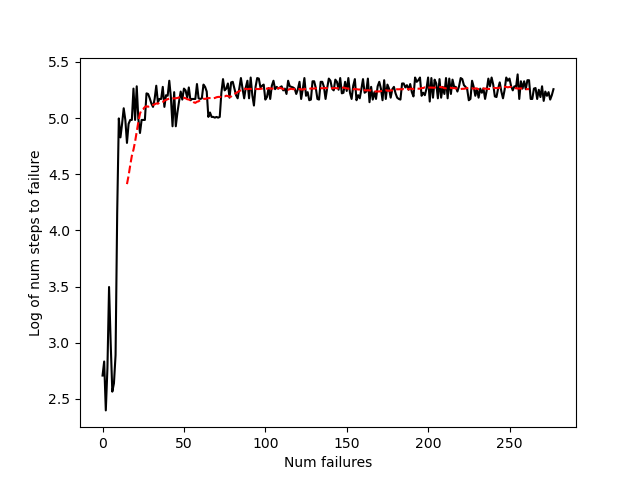
\includegraphics[width=\linewidth]{learning0}
		\caption{Seed 0. Converged in 278 iterations.}
	\end{subfigure}
	\begin{subfigure}[H]{0.45\linewidth}
		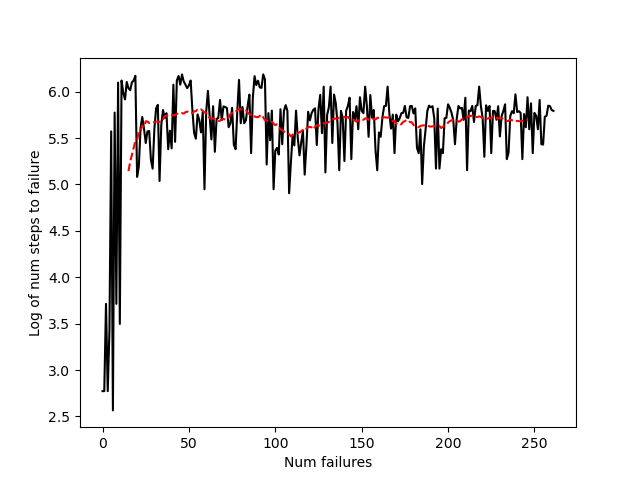
\includegraphics[width=\linewidth]{learning1}
		\caption{Seed 1. Converged in 262 iterations.}
	\end{subfigure}
	\begin{subfigure}[H]{0.45\linewidth}
		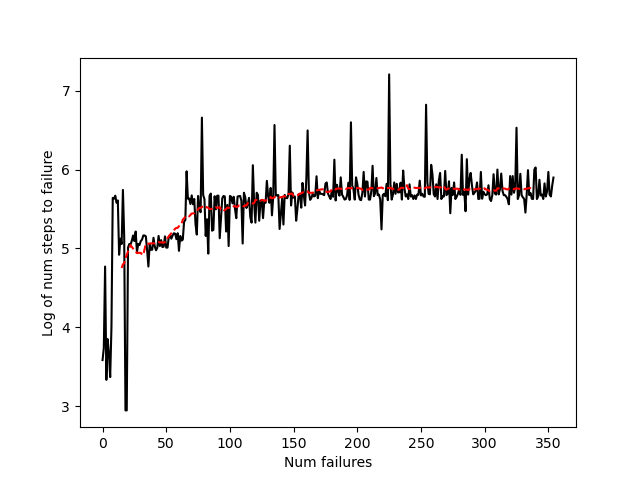
\includegraphics[width=\linewidth]{learning2}
		\caption{Seed 2. Converged in 355 iterations.}
	\end{subfigure}
	\begin{subfigure}[H]{0.45\linewidth}
		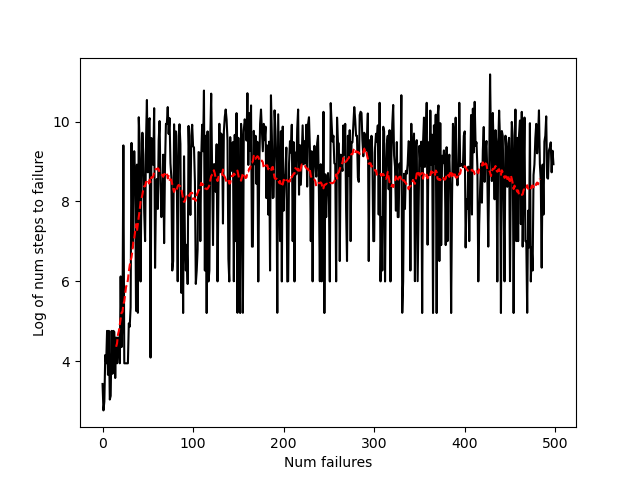
\includegraphics[width=\linewidth]{learning3}
		\caption{Seed 3. Didn't converged after 500 iters.}
	\end{subfigure}
	\caption{The learning process of the inverted pendulum problem with different seeds.}
\end{figure}
The learning curves are very different for different seeds. At the default seed 0, our model succeeded to converge after 278 iterations. The learning curve of seed 3 looks extremely noisy and therefore it fails to converge even after 500 iterations. Yet, the duration of a trial is about 7 times longer in average when using seed 3 than those of other seeds. This implies that our algorithm is very sensitive to exploration strategies and the quality of learned policies can vary significantly. Illustration of a trial according to our learned policy with default seed 0 can be found in \href{https://github.com/huyfam/CS229-solutions-summer-2019-2020/blob/main/psets/ps3/src/cartpole/simulation.gif}{here}.

\end{answer}
